\documentclass{beamer}
%\documentclass[xcolor=dvipsnames]{beamer}
\usepackage[spanish]{babel}
\usepackage[utf8]{inputenc}
\usepackage{graphicx}

\newcommand{\beamer}{\textsc{beamer}}
\newtheorem{definicion}{Definición}
\newtheorem{ejemplo}{Ejemplo}

%%%%%%%%%%%%%%%%%%%%%%%%%%%%%%%%%%%%%%%%%%%%%%%%%%%%%%%%%%%%%%%%%%%%%%%%%%%%%%%
\title[Método Simpson]{Integración numérica de Simpson}
\author[Samuel e Iván]{Samuel Santos Lucas Castilla \\
                       Iván Trujillo Trujillo}
\institute[ULL]{Universidad de La Laguna}
\date[17-05-2013]{17 de mayo de 2013}
%%%%%%%%%%%%%%%%%%%%%%%%%%%%%%%%%%%%%%%%%%%%%%%%%%%%%%%%%%%%%%%%%%%%%%%%%%%%%%%

\usetheme{Madrid}

%%%%%%%%%%%%%%%%%%%%%%%%%%%%%%%%%%%%%%%%%%%%%%%%%%%%%%%%%%%%%%%%%%%%%%%%%%%%%%%
\definecolor{pantone254}{RGB}{122,59,122}
\definecolor{pantone3015}{RGB}{0,88,147}
\definecolor{pantone432}{RGB}{56,61,66}
\setbeamercolor*{palette primary}{use=structure,fg=white,bg=pantone254}
\setbeamercolor*{palette secondary}{use=structure,fg=white,bg=pantone3015}
\setbeamercolor*{palette tertiary}{use=structure,fg=white,bg=pantone432}
\setbeamercolor*{palette sidebar primary}{use=structure,fg=pantone254}
\setbeamercolor*{palette sidebar tertiary}{use=structure,fg=pantone3015}
\setbeamercolor*{block title}{bg=pantone3015,fg=white}
\setbeamercolor*{alerted text}{fg=pantone432}
\setbeamercolor*{item projected}{fg=pantone254}
\setbeamercolor*{section in toc shaded}{use=structure,fg=structure.fg}
\setbeamercolor*{section in toc}{fg=pantone3015}
\setbeamercolor*{subsection in toc shaded}{fg=pantone3015}
\setbeamercolor*{subsection in toc}{fg=pantone432}

%%%%%%%%%%%%%%%%%%%%%%%%%%%%%%%%%%%%%%%%%%%%%%%%%%%%%%%%%%%%%%%%%%%%%%%%%%%%%%%
\begin{document}
  
%++++++++++++++++++++++++++++++++++++++++++++++++++++++++++++++++++++++++++++++  
\begin{frame}

  
\includegraphics[width=0.15\textwidth]{img/ullesc.eps}
  \hspace*{7.5cm}
  
\includegraphics[width=0.16\textwidth]{img/fmatesc.eps}
  \titlepage

  \begin{scriptsize}
    \begin{center}
     Facultad de Matemáticas \\
     Universidad de La Laguna
    \end{center}
  \end{scriptsize}

\end{frame}
%++++++++++++++++++++++++++++++++++++++++++++++++++++++++++++++++++++++++++++++  

%++++++++++++++++++++++++++++++++++++++++++++++++++++++++++++++++++++++++++++++  
\begin{frame}
  \frametitle{Índice}  
  \tableofcontents[pausesections]
\end{frame}
%++++++++++++++++++++++++++++++++++++++++++++++++++++++++++++++++++++++++++++++  


\section{Motivación y Objetivos}


%++++++++++++++++++++++++++++++++++++++++++++++++++++++++++++++++++++++++++++++  
\begin{frame}

\frametitle{Motivación}

\begin{definicion}
...
\end{definicion}

\end{frame}
%++++++++++++++++++++++++++++++++++++++++++++++++++++++++++++++++++++++++++++++  

%++++++++++++++++++++++++++++++++++++++++++++++++++++++++++++++++++++++++++++++  
\begin{frame}

\frametitle{Objetivos }

\begin{block}{Ejemplo}
  \begin{itemize}
  \item
   Implementar un programa en Python que sea capaz de resolver el problema del cálculo del área bajo una función conocida en un 
   intervalo cerrado.
  \pause
  \item
   Entender los conceptos básicos de la integración aproximada empleando el método de Simpson, para posteriormente, saber emplearlos
   en Python.

  \end{itemize}
\end{block}

\end{frame}
%++++++++++++++++++++++++++++++++++++++++++++++++++++++++++++++++++++++++++++++  

\section{Fundamentos Teóricos}

\begin{frame}
\frametitle{Fundamentos Teóricos}
	El método de Simpson se trata de un procedimiento por el cual se obtiene una estimación más exacta de una integral. Para ello se 
utilizan polinomios de orden superior para conectar los puntos, concretamente de orden 2, es decir, de la forma: $ ax^2 + bx + c $.

	En este procedimiento, se toma el intervalo de anchura 2h, comprendido entre $x_{i}$ y $ x_{i+2} $, y se sustituye la funcion f(x) por la parábola que pasa por los puntos $ (x_{i},y_{i}) $, $ (x_{i+1},y_{i+1}) $, y $ (x_{i+2},y_{i+2}) $.

\end{frame}

\begin{frame}
\frametitle{Fundamentos Teóricos}
\subsection{Deducción del modelo a partir de la ecuación de la parábola}
Para demostrar el método de Simpson hay que asumir que cada sub área es un pequeño arco de parábola de la forma $ ax^2 + bx + c $ cuyos límites son los siguientes: límite inferior en -h , límite superior en h y por ende la mitad de la sub área se encontrará en el punto 0, tal y como se ve en la figura 2.
	
%\begin{center}
%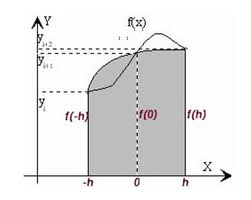
\includegraphics[width=0.2\textwidth]{mem/images/imagen2}\\[0.25cm]
%\end{center}	
	
		Se procede a la integración de dicho arco de parábola entre los límites descritos:
		
		\[ \int_{-h}^{h}\left(\textup{a}x^2 + \textup{b}x + \textup{c}\right)\textup{d}x=\left[\frac{\textup{a}x^{3}}
		{3}+\frac{\textup{b}x^{2}}{2}+\textup{c}x\right]_{-h}^{h} \] 
		
		Si se reemplazan cada uno de los límites y se quitan los corchetes se obtiene lo siguiente:
		
		\[\frac{\textup{a}\textup{h}^3}{3} + \frac{\textup{b}\textup{h}^2}{2} + \textup{c}\textup{h} + \frac{\textup{a}\textup{h}^3}{3} 
		-  \frac{\textup{b}\textup{h}^2}{2} + \textup{c}\textup{h}=2\frac{\textup{a}\textup{h}^3}{2\textup{c}\textup{h}}\]
		
		Y si se simplifica obtenemos la ecuación 1 que se muestra a continuación:
		
		Ecuación 1: \[\int_{-h}^{h}\left((\textup{a}x^2 + \textup{b}x + \textup{c}\right)\textup{d}x=\frac{\textup{h}}
		{3}\left[2\textup{a}\textup{h}^2  +  6\textup{c}\right]\]
		
%\begin{center}
%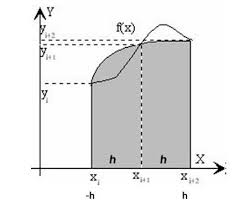
\includegraphics[width=0.2\textwidth]{mem/images/imagen3}\\[0.25cm]
%\end{center}
	
\end{frame}

\begin{frame}
\frametitle{Fundamentos Teóricos}
	En la figura 3 se observa, respecto a las notaciones, las siguientes igualdades:
	
	\begin{itemize}
    \item $ \textup{f}x_{i}=y_{i}=\textup{f}\textup{(-h)} $
    \pause
    \item $ \textup{f}x_{i+1}=y_{i+1}=\textup{f}(0) $
    \pause
    \item $ \textup{f}x_{i+2}=y_{i+2}=\textup{f}\textup{(h)} $
    \pause
    \end{itemize}


    Entonces se podría obtener, evaluando la ecuación general $ \textup{a}x^2 + \textup{b}x + \textup{c} $ en cada uno de los puntos de la sub área [-h,0,h], el siguiente sistema de ecuaciones:
	
	$ \textup{f}\textup{(-h)}=\textup{a}\textup{h}^2 - \textup{b}\textup{h} + \textup{c} $, se puede tomar esta altura como 
	$ y_{0}=\textup{f}x_{i}$.
	
	
	$ \textup{f}(0)=\textup{c} $, se toma esta altura como $ y_{1}=\textup{f}x_{i+1} $.
	
	
	$ \textup{f}\textup{(h)}=\textup{a}\textup{h}^2 + \textup{b}\textup{h} + \textup{c} $, y esta altura como $ 
	y_{2}=\textup{f}x_{i+2}$.

\end{frame}

\begin{frame}
\frametitle{Fundamentos Teóricos}
	De lo anterior se puede deducir las siguientes dos ecuaciones:

	
	Ecuación 2: $ y_{0} + y_{2} = 2\textup{a}\textup{h}^2 + 2\textup{c} $.

	
	Ecuación 3: $ y_{i}=\textup{c} $.

	
	Si se vuelve a la Ecuación 1 se ve que se puede expresar igualmente de la siguiente forma:
	
	Ecuación 4: $ \int_{-h}^{h}\left(\textup{a}x^2 + \textup{b}x + \textup{c}\right)\textup{d}x = \frac{\textup{h}}
	{3}\left[2\textup{a}\textup{h}^2 + 2\textup{c} + 4\textup{c}\right] $.

		
	Si se remplaza las ecuanciones 2 y 3 en la Ecuación 4 se obtiene que:

	
	Ecuación 5: $ \int_{-h}^{h}\left(\textup{a}x^2 + \textup{b}x + \textup{c}\right)\textup{d}x = \frac{\textup{h}}{3}\left[y_{0} + 
	4y_{1} + y_{2}\right] = \textup{A}_{1}  $.

\end{frame}

\begin{frame}
\frametitle{Fundamentos Teóricos}
	Ahora se interpreta la Ecuación 5 con base en la sub área seleccionada $\textup{A}_{1}$ para el desarrollo del método de Simpson, se diría que el área del segmento es igual a la suma de la altura o función evaluada en el lado izquierdo más cuatro veces la función evaluada en la parte central de la sub área más la función evaluada en el lado derecho de la sub área, y todo ello multiplicado por el ancho del sub área y dividido por 3.
	
	Si se toma a y b como $ x_{0} $ y $ x_{2} $, y $ \textup{f}_{i}\left(x_{i}\right) $ se representa mediante un polinomio de Lagrange de segundo orden, luego la integral que quedaría sería la siguiente:
	
	\[ \textup{I} = \int_{x_{0}}^{x_{2}}\left[\frac{(x - x_{1})(x - x_{2})}{(x_{0} - x_{1})(x_{0} - x_{2})}\textup{f}(x_{0}) + \frac{(x 
	- x_{1})(x - x_{2})}{(x_{1} - x_{0})(x_{1} - x_{2})}\textup{f}(x_{1}) + \frac{(x - x_{1})(x - x_{1})}{(x_{2} - x_{0})(x_{2} - 
	x_{1})}\textup{f}(x_{2})\right]\textup{d}x\]	
	
	Después de integrar y de reordenar los términos, se obtiene como resultado la siguiente ecuación:
	
	\[\textup{I} = \left(\textup{b}-\textup{a}\right)\frac{\textup{f}\left(x_{0}\right) + 4\textup{f}\left(x_{1}\right) + \textup{f}\left(x_{2}\right)}{6}\]

\end{frame}

%++++++++++++++++++++++++++++++++++++++++++++++++++++++++++++++++++++++++++++++  

\section{Procedimiento experimental}

\begin{frame}
\frametitle{Procedimiento experimental}

	A continuación se procederá a describir el experimento realizado, los materiales empleados para su realización,
los resultados obtenidos y a analizar dichos resultados.

\end{frame}
%++++++++++++++++++++++++++++++++++++++++++++++++++++++++++++++++++++++++++++++  

\subsection{Descripción de los experimentos}

%++++++++++++++++++++++++++++++++++++++++++++++++++++++++++++++++++++++++++++++  
\begin{frame}
\frametitle{Descripción de los experimentos}
	En este experimentos se lleva a cabo la implentación e interpretación de un programa en Python que
 este capacitado para calcular el valor de una integral definida en un intervalo cerrado, una aproximación por 
 el método de Simpson, halle los errores relativo y absoluto entre los dos valores obtenidos y realice la representación
gráfica de la función que se desea integrar y la parábola generada por el método utilizado
para su aproximación.
 	
 \begin{enumerate}
    \item La función con la que se ha trabajado es: $f(x) = \frac{1}{1+e^{x}}$.
    \pause
    \item Y el intervalo en la se definine es: $x \in [1, 6]$.
    \pause
    \item Considerimos f'(x) como $\ln{e^{x}} - \ln({e^{x}+1)}$
    \pause
    \item La parabola ha representar viene dado por los puntos:
    \begin{enumerate}
      \item f(a)
      \pause
      \item f(b)
      \pause
      \item f($\frac{a+b}{2}$)
    \end{enumerate}
    \pause
    \item Por tanto, la ecuación obtenida es: $y = 0.0169x^2 - 0.17x + 0.422 $
      
 \end{enumerate}
\end{frame}
%++++++++++++++++++++++++++++++++++++++++++++++++++++++++++++++++++++++++++++++  

\subsection{Descripción del material}
%++++++++++++++++++++++++++++++++++++++++++++++++++++++++++++++++++++++++++++++  
\begin{frame}
\frametitle{Hardware y Software}

\begin{ejemplo}
  \begin{enumerate}
    \item
      Descripción del hardware 
      \pause

    \item
      Descripción del software 
  \end{enumerate}
\end{ejemplo}

\end{frame}
%++++++++++++++++++++++++++++++++++++++++++++++++++++++++++++++++++++++++++++++  

\subsection{Resultados obtenidos}
%++++++++++++++++++++++++++++++++++++++++++++++++++++++++++++++++++++++++++++++  
\begin{frame}
\frametitle{Resultados obtenidos}

%------------------------------------------------------------------------------
%--------------------------------------------------------------------------
\begin{table}[!ht]
\begin{center}
\begin{tabular}{|c|c|} \hline 
\textbf{Tiempo  } & \textbf{Velocidad} \\ 
\textbf{($\pm$ 0.001 s)} & \textbf{($\pm$ 0.1 m/s)} \\ \hline \hline
1.234 &
67.8
\\
\hline

2.345 &
78.9
\\
\hline

3.456 &
89.1
\\
\hline

4.567 &
91.2
\\
\hline

\end{tabular}
\end{center}
\caption{Resultados experimentales de tiempo (s) y velocidad (m/s)}
\label{tab:1}
\end{table}


%------------------------------------------------------------------------------

\end{frame}
%++++++++++++++++++++++++++++++++++++++++++++++++++++++++++++++++++++++++++++++  


\subsection{Análisis de los resultados}
%++++++++++++++++++++++++++++++++++++++++++++++++++++++++++++++++++++++++++++++  
\begin{frame}
\frametitle{Análisis de los resultados}

%------------------------------------------------------------------------------
\begin{figure}[!th]
\begin{center}
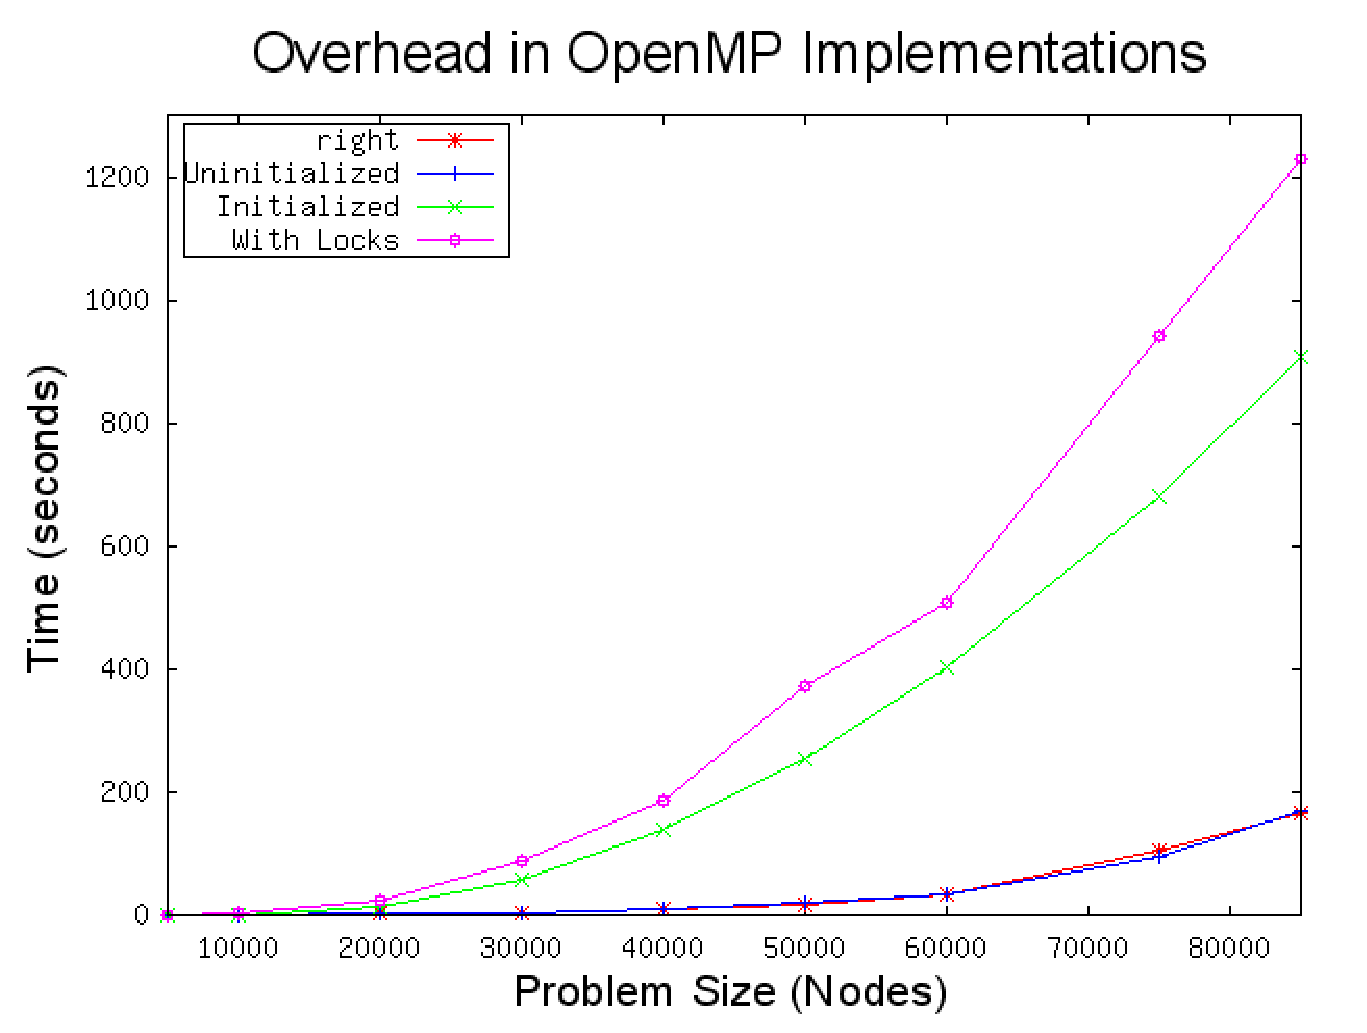
\includegraphics[width=0.75\textwidth]{img/figura1.eps}
\caption{Ejemplo de figura}
\label{fig:1}
\end{center}
\end{figure}
%------------------------------------------------------------------------------

\end{frame}
%++++++++++++++++++++++++++++++++++++++++++++++++++++++++++++++++++++++++++++++  


\section{Conclusiones}

%++++++++++++++++++++++++++++++++++++++++++++++++++++++++++++++++++++++++++++++  
\begin{frame}
\frametitle{Conclusiones}

\begin{ejemplo}
  \begin{enumerate}
    \item
      Conclusión 1
      \pause
    \item
      Conclusión 2
  \end{enumerate}
\end{ejemplo}

\end{frame}
%++++++++++++++++++++++++++++++++++++++++++++++++++++++++++++++++++++++++++++++  

%++++++++++++++++++++++++++++++++++++++++++++++++++++++++++++++++++++++++++++++  
\begin{frame}
  \frametitle{Bibliografía}

  \begin{thebibliography}{10}

    \beamertemplatebookbibitems
    \bibitem[Plan Estudios, 2011]{plan}  
    Documento de verificación del grado. 
    (2011) 

    \beamertemplatebookbibitems
    \bibitem[Guía Docente, 2013]{guia}  
    Guía docente. 
    (2013) 
    {\small $http://eguia.ull.es/matematicas/query.php?codigo=299341201$}

    \beamertemplatebookbibitems
    \bibitem[URL: CTAN]{latex} 
    CTAN. {\small $http://www.ctan.org/$}

    \beamertemplatebookbibitems
    \bibitem[Tantau, 2005]{beamer} 
    Tantau, Till. 
    \emph{User's Guide to the \beamer{} Class, Version 3.06, 2005} 
    {\small $http://ctang.tug.org/tex-archive/macros/latex/contrib/beamer$}


  \end{thebibliography}
\end{frame}


%++++++++++++++++++++++++++++++++++++++++++++++++++++++++++++++++++++++++++++++  

\end{document}
